\documentclass{article}
\usepackage[margin=1in,bottom=1.5in,footskip=1in]{geometry}

\usepackage{multicol}
\usepackage{fancyhdr}
\usepackage{lastpage}
\pagestyle{fancy}
\fancyhf{}
\lfoot{\thepage/\pageref*{LastPage}}
\rfoot{
\includegraphics[height=5em]{square_bw}}
\renewcommand{\headrulewidth}{0pt}
\renewcommand{\footrulewidth}{0pt}



\newcommand{\morseDit}{{\large .}}
\newcommand{\morseDah}{{\large -}}

\usepackage[puttinydots]{braille}


% set font encoding for PDFLaTeX, XeLaTeX, or LuaTeX
\usepackage{ifxetex,ifluatex}
\if\ifxetex T\else\ifluatex T\else F\fi\fi T%
  \usepackage{fontspec}
\else
  \usepackage[T1]{fontenc}
  \usepackage[utf8]{inputenc}
  \usepackage{lmodern}
\fi
\usepackage{tgadventor}
\renewcommand*\familydefault{\sfdefault} %% Only if the base font of the document is to be sans serif

\usepackage{hyperref}
\usepackage{xcolor}
\definecolor{mygray}{gray}{0.8}


\usepackage{pifont}
\DeclareFontFamily{U}{dice3d}{}
\DeclareFontShape{U}{dice3d}{m}{n}{<-> s*[20] dice3d}{}
\usepackage{tikz}

\newcommand{\die}[2]{
\begin{scope}[shift={(#1)}]
\fill[color=white] (0,0.2) -- (0.2,0) -- (0.9,0) -- (0.95,0.1) -- (0.95,1)
  -- (0.03,3.65) -- (-0.9,3.7) -- (-0.9,2.85);
\node[anchor=south west] at (0,0) {\usefont{U}{dice3d}{m}{n}{#2}};
\end{scope}
}
\newcommand{\diegridcustom}[2]{
\begin{tikzpicture}[every node/.style={inner sep=0,outer sep=0},scale=1.34,y={(0.35355,0.35355,0)}]
\foreach \x in {0,1,...,#2} {
\draw[thick] (0,\x) -- (#2,\x);
\draw[thick] (\x,0) -- (\x,#2);
}
#1
\end{tikzpicture}
}
\newcommand{\diegrid}[1]{\diegridcustom{#1}{4}}
\newcommand{\diagramEight}{
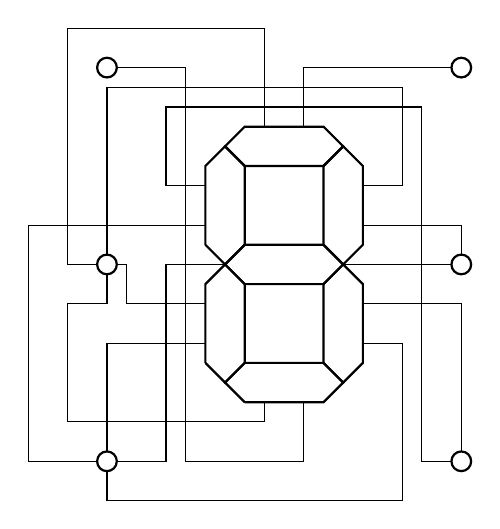
\begin{tikzpicture}[scale=0.25]
%\draw[color=black!20,step=1] (-6,-4) grid (14,18);
\begin{scope}
\draw[thick] (2,0) -- (6,0) -- (7,1) -- (6,2) -- (2,2) -- (1,1) -- (2,0);
\end{scope}
\begin{scope}[shift={(0,6)}]
\draw[thick] (2,0) -- (6,0) -- (7,1) -- (6,2) -- (2,2) -- (1,1) -- (2,0);
\end{scope}
\begin{scope}[shift={(0,12)}]
\draw[thick] (2,0) -- (6,0) -- (7,1) -- (6,2) -- (2,2) -- (1,1) -- (2,0);
\end{scope}
\begin{scope}
\draw[thick] (0,2) -- (1,1) -- (2,2) -- (2,6) -- (1,7) -- (0,6) -- (0,2);
\end{scope}
\begin{scope}[shift={(6,0)}]
\draw[thick] (0,2) -- (1,1) -- (2,2) -- (2,6) -- (1,7) -- (0,6) -- (0,2);
\end{scope}
\begin{scope}[shift={(0,6)}]
\draw[thick] (0,2) -- (1,1) -- (2,2) -- (2,6) -- (1,7) -- (0,6) -- (0,2);
\end{scope}
\begin{scope}[shift={(6,6)}]
\draw[thick] (0,2) -- (1,1) -- (2,2) -- (2,6) -- (1,7) -- (0,6) -- (0,2);
\end{scope}
\draw (-5,-3) -- (-2,-3) -- (-2,7) -- (1,7);
\draw (-5,-3) -- (-9,-3) -- (-9,9) -- (0,9);
\draw (-5,-3) -- (-5,-5) -- (10,-5) -- (10,3) -- (8,3);
\draw (-5,-3) -- (-5,3) -- (0,3);
\draw (-5,7) -- (-5,5) -- (-7,5) -- (-7,-1) -- (3,-1) -- (3,0);
\draw (-5,7) -- (-7,7) -- (-7,19) -- (3,19) -- (3,14);
\draw (-5,7) -- (-4,7) -- (-4,5) -- (0,5);
\draw (-5,7) -- (-5,16) -- (10,16) -- (10,11) -- (8,11);
\draw (-5,17) -- (-1,17) -- (-1,-3) -- (5,-3) -- (5,0);
\draw (13,17) -- (5,17) -- (5,14);
\draw (13,7) -- (7,7);
\draw (13,7) -- (13,9) -- (8,9);
\draw (13,-3) -- (11,-3) -- (11,15) -- (-2,15) -- (-2,11) -- (0,11);
\draw (13,-3) -- (13,5) -- (8,5);
\draw[thick,fill=white] (-5,-3) circle (0.5);
\draw[thick,fill=white] (-5,7) circle (0.5);
\draw[thick,fill=white] (-5,17) circle (0.5);
\draw[thick,fill=white] (13,-3) circle (0.5);
\draw[thick,fill=white] (13,7) circle (0.5);
\draw[thick,fill=white] (13,17) circle (0.5);
\end{tikzpicture}
}

\newcommand{\dominoLetter}[1]{
\includegraphics[width=0.12\linewidth]{early-drafts/dominoRally/letter#1.pdf}
\hspace{0.03\linewidth}
}
\newcommand{\undominoLetter}[1]{
\includegraphics[width=0.12\linewidth]{early-drafts/dominoRally/letter#1Fake.pdf}
\hspace{0.03\linewidth}
}

\newcommand{\clue}[1]{#1}
%\renewcommand{\clue}[1]{}

\newcommand{\puzzleTitle}[1]{
\begin{center}
{\Large \texttt{#1}}
\end{center}
}

\title{Challenge21 draft}
\author{MaPP}


% Enable SageTeX to run SageMath code right inside this LaTeX file.
% http://doc.sagemath.org/html/en/tutorial/sagetex.html
% \usepackage{sagetex}

% Enable PythonTeX to run Python – https://ctan.org/pkg/pythontex
% \usepackage{pythontex}

\begin{document}
%\maketitle

\thispagestyle{empty}
\begin{center}

\includegraphics[width=0.8\linewidth]{banner_bw}

\Large MaPP Challenge '21: \textit{Enter the Array}

%Player Book
\end{center}

\vspace{1in}

%\noindent
%Print a copy of this book for each
%player before your game begins, or set up
%each page in a virtual whiteboard.
%You can look through these pages before the game begins,
%but you'll need the clues provided in the ClueKeeper app
%to make much progress.

\vspace{1em}

\noindent
%Have fun!

\vfill

{\footnotesize PDF last updated: \today}

\newpage

\puzzleTitle{Anders}

\vfill

\begin{center}\Large
\begin{tabular}{c||c|c|c||c|c|c||c|c|c||c}
  & \phantom3\(\downarrow\) & \phantom2\(\downarrow\) & \phantom4\(\downarrow\) & \phantom1\(\downarrow\) & \phantom2\(\downarrow\) & \phantom5\(\downarrow\) & \phantom3\(\downarrow\) & \phantom3\(\downarrow\) & \phantom3\(\downarrow\) &   \\\hline\hline
\phantom3\(\rightarrow\) &   & \color{mygray}{$\clubsuit$} & 1 &   &   &   & 5 &   &   & \(\leftarrow\)\phantom3 \\\hline
\phantom2\(\rightarrow\) &   &   & 5 &   & \color{mygray}{$\heartsuit$} &   & 2 &   & \color{mygray}{$\clubsuit$} & \(\leftarrow\)\phantom3 \\\hline
\phantom4\(\rightarrow\) & 3 & 4 & 8 & 7 & 2 & 5 & 1 & 9 & 6 & \(\leftarrow\)\phantom2 \\\hline\hline
\phantom1\(\rightarrow\) &   &   & 6 & \color{mygray}{$\clubsuit$} &   &   & 7 &   &   & \(\leftarrow\)\phantom5 \\\hline
\phantom3\(\rightarrow\) & \color{mygray}{$\diamondsuit$} &   & 2 & \color{mygray}{$\heartsuit$} &   & \color{mygray}{$\spadesuit$} & 3 & \color{mygray}{$\nabla$} &   & \(\leftarrow\)\phantom2 \\\hline
\phantom2\(\rightarrow\) &   & \color{mygray}{$\star$} & 7 &   &   &   & 9 &   & \color{mygray}{$\diamondsuit$} & \(\leftarrow\)\phantom3 \\\hline\hline
\phantom4\(\rightarrow\) & 6 & 7 & 3 & 5 & 1 & 8 & 4 & 2 & 9 & \(\leftarrow\)\phantom1 \\\hline
\phantom3\(\rightarrow\) &   & \color{mygray}{$\heartsuit$} & 4 &   & \color{mygray}{$\nabla$} &   & 6 & \color{mygray}{$\spadesuit$} &   & \(\leftarrow\)\phantom3 \\\hline
\phantom3\(\rightarrow\) &   &   & 9 &   &   & \color{mygray}{$\diamondsuit$} & 8 &   &   & \(\leftarrow\)\phantom4 \\\hline\hline
  & \phantom5\(\uparrow\) & \phantom3\(\uparrow\) & \phantom1\(\uparrow\) & \phantom3\(\uparrow\) & \phantom3\(\uparrow\) & \phantom2\(\uparrow\) & \phantom2\(\uparrow\) & \phantom2\(\uparrow\) & \phantom2\(\uparrow\) &
\end{tabular}
\end{center}

\vspace{3em}

\begin{center}
\begin{tabular}{c c c c c c}
 & \\
\underline{\phantom{xyz}} & \underline{\phantom{xyz}} & \underline{\phantom{xyz}} & \underline{\phantom{xyz}} & \underline{\phantom{xyz}} & \underline{\phantom{xyz}}\\
$\nabla$ & $\heartsuit$ & $\clubsuit$ & $\diamondsuit$ & $\star$ & $\spadesuit$
\end{tabular}
\end{center}

\vfill

\newpage


\clue{
Anders' Clue

The Designer is obsessed with the layout of human cities.
They have often confided in me their desire to create the
"perfect Sudoku
City". In this city, every building is between one and nine levels
tall, and the heights of the buildings in each row, column, and
3x3 subsquare include exactly one building of each height.

There's a bit more to it, however. They also have insisted that
this perfect city satisfy certain "boundary conditions". I'm
not sure what they mean, but hopefully you can puzzle it out by using
the known heights in the third and seventh rows and columns.

Of course, even once the city layout is known, there's still the matter
of extracting the Designer's hidden password...

\begin{center}\Large
\begin{tabular}{c||c|c|c||c|c|c||c|c|c||c}
  & 3\(\downarrow\) & 2\(\downarrow\) & 4\(\downarrow\) & 1\(\downarrow\) & 2\(\downarrow\) & 5\(\downarrow\) & 3\(\downarrow\) & 3\(\downarrow\) & 3\(\downarrow\) &   \\\hline\hline
3\(\rightarrow\) &   & \color{mygray}{$\clubsuit$} & 1 &   &   &   & 5 &   &   & \(\leftarrow\)3 \\\hline
2\(\rightarrow\) &   &   & 5 &   & \color{mygray}{$\heartsuit$} &   & 2 &   & \color{mygray}{$\clubsuit$} & \(\leftarrow\)3 \\\hline
4\(\rightarrow\) & 3 & 4 & 8 & 7 & 2 & 5 & 1 & 9 & 6 & \(\leftarrow\)2 \\\hline\hline
1\(\rightarrow\) &   &   & 6 & \color{mygray}{$\clubsuit$} &   &   & 7 &   &   & \(\leftarrow\)5 \\\hline
3\(\rightarrow\) & \color{mygray}{$\diamondsuit$} &   & 2 & \color{mygray}{$\heartsuit$} &   & \color{mygray}{$\spadesuit$} & 3 & \color{mygray}{$\nabla$} &   & \(\leftarrow\)2 \\\hline
2\(\rightarrow\) &   & \color{mygray}{$\star$} & 7 &   &   &   & 9 &   & \color{mygray}{$\diamondsuit$} & \(\leftarrow\)3 \\\hline\hline
4\(\rightarrow\) & 6 & 7 & 3 & 5 & 1 & 8 & 4 & 2 & 9 & \(\leftarrow\)1 \\\hline
3\(\rightarrow\) &   & \color{mygray}{$\heartsuit$} & 4 &   & \color{mygray}{$\nabla$} &   & 6 & \color{mygray}{$\spadesuit$} &   & \(\leftarrow\)3 \\\hline
3\(\rightarrow\) &   &   & 9 &   &   & \color{mygray}{$\diamondsuit$} & 8 &   &   & \(\leftarrow\)4 \\\hline\hline
  & 5\(\uparrow\) & 3\(\uparrow\) & 1\(\uparrow\) & 3\(\uparrow\) & 3\(\uparrow\) & 2\(\uparrow\) & 2\(\uparrow\) & 2\(\uparrow\) & 2\(\uparrow\) &
\end{tabular}
\end{center}
}


\newpage

\puzzleTitle{Garcia}

\vfill

\newcounter{XPos}

\newcommand{\phCommandColumn}[5]{
\fill[color=lightgray] (\theXPos,3) rectangle +(1,2);
\draw[step=1] (\theXPos,0) grid +(1,5);
\draw[very thick] (\theXPos,3) -- +(1,0);
\node at (\theXPos.5,4.5) {#1};
\node at (\theXPos.5,3.5) {#2};
\node at (\theXPos.5,2.5) {#3};
\node at (\theXPos.5,1.5) {#4};
\node at (\theXPos.5,0.5) {#5};
\stepcounter{XPos}
}

\begin{center}
  \begin{tikzpicture}[x=1.5em,y=1.5em]
    \phCommandColumn{ 1}{ }{A}{\( \rightarrow \)}{10}
    \phCommandColumn{ 1}{G}{ }{\(  \leftarrow \)}{ 8}
    \phCommandColumn{ 1}{J}{V}{\( \rightarrow \)}{ 6}
    \phCommandColumn{ 1}{X}{ }{\( \rightarrow \)}{20}
    \phCommandColumn{ 2}{ }{S}{\(  \leftarrow \)}{11}
    \phCommandColumn{ 2}{A}{A}{\( \rightarrow \)}{14}
    \phCommandColumn{ 2}{E}{F}{\( \rightarrow \)}{ 3}
    \phCommandColumn{ 2}{V}{ }{\( \rightarrow \)}{ 7}
    \phCommandColumn{ 3}{ }{ }{\( \rightarrow \)}{ 2}
    \phCommandColumn{ 3}{E}{R}{\( \rightarrow \)}{ 4}
    \phCommandColumn{ 3}{X}{ }{\(  \leftarrow \)}{17}
    \phCommandColumn{ 3}{Y}{G}{\( \rightarrow \)}{ 1}
    \phCommandColumn{ 4}{ }{ }{\( \rightarrow \)}{ 3}
    \phCommandColumn{ 4}{A}{A}{\(  \leftarrow \)}{13}
    \phCommandColumn{ 4}{J}{G}{\(  \leftarrow \)}{ 1}
    \phCommandColumn{ 4}{E}{E}{\( \rightarrow \)}{ 4}
    \phCommandColumn{ 5}{ }{A}{\( \rightarrow \)}{ 4}
    \phCommandColumn{ 5}{A}{A}{\(  \leftarrow \)}{13}
    \phCommandColumn{ 5}{B}{O}{\(  \leftarrow \)}{19}
    \phCommandColumn{ 5}{J}{Y}{\(  \leftarrow \)}{ 1}
  \end{tikzpicture}
\end{center}
\begin{center}
  \begin{tikzpicture}[x=1.5em,y=1.5em]
    \phCommandColumn{ 6}{ }{ }{\( \rightarrow \)}{ 5}
    \phCommandColumn{ 6}{B}{ }{\( \rightarrow \)}{11}
    \phCommandColumn{ 6}{J}{X}{\(  \leftarrow \)}{ 6}
    \phCommandColumn{ 6}{O}{ }{\( \rightarrow \)}{22}
    \phCommandColumn{ 7}{ }{ }{\( \rightarrow \)}{ 6}
    \phCommandColumn{ 7}{G}{J}{\(  \leftarrow \)}{20}
    \phCommandColumn{ 7}{V}{ }{\(  \leftarrow \)}{13}
    \phCommandColumn{ 7}{Y}{B}{\(  \leftarrow \)}{ 6}
    \phCommandColumn{ 8}{ }{ }{\( \rightarrow \)}{ 7}
    \phCommandColumn{ 8}{B}{ }{\( \rightarrow \)}{ 1}
    \phCommandColumn{ 8}{V}{G}{\( \rightarrow \)}{14}
    \phCommandColumn{ 8}{X}{J}{\(  \leftarrow \)}{11}
    \phCommandColumn{ 9}{ }{ }{\( \rightarrow \)}{ 8}
    \phCommandColumn{ 9}{G}{B}{\(  \leftarrow \)}{ 2}
    \phCommandColumn{ 9}{J}{V}{\( \rightarrow \)}{17}
    \phCommandColumn{ 9}{O}{X}{\(  \leftarrow \)}{12}
    \phCommandColumn{10}{ }{ }{\( \rightarrow \)}{ 9}
    \phCommandColumn{10}{B}{G}{\(  \leftarrow \)}{ 3}
    \phCommandColumn{10}{G}{B}{\( \rightarrow \)}{11}
    \phCommandColumn{10}{V}{X}{\( \rightarrow \)}{16}
    \phCommandColumn{11}{ }{ }{\(  \leftarrow \)}{11}
    \phCommandColumn{11}{A}{A}{\(  \leftarrow \)}{12}
    \phCommandColumn{11}{X}{ }{\( \rightarrow \)}{17}
    \phCommandColumn{11}{Y}{ }{\(  \leftarrow \)}{ 4}
  \end{tikzpicture}
\end{center}
\begin{center}
  \begin{tikzpicture}[x=1.5em,y=1.5em]
    \phCommandColumn{12}{ }{E}{\(  \leftarrow \)}{12}
    \phCommandColumn{12}{G}{Y}{\(  \leftarrow \)}{ 8}
    \phCommandColumn{12}{A}{A}{\( \rightarrow \)}{ 2}
    \phCommandColumn{12}{Z}{ }{\( \rightarrow \)}{17}
    \phCommandColumn{13}{ }{B}{\( \rightarrow \)}{10}
    \phCommandColumn{13}{E}{M}{\( \rightarrow \)}{ 2}
    \phCommandColumn{13}{J}{ }{\( \rightarrow \)}{ 2}
    \phCommandColumn{13}{S}{S}{\(  \leftarrow \)}{21}
    \phCommandColumn{14}{ }{ }{\( \rightarrow \)}{14}
    \phCommandColumn{14}{V}{ }{\(  \leftarrow \)}{19}
    \phCommandColumn{14}{S}{S}{\( \rightarrow \)}{15}
    \phCommandColumn{14}{Y}{B}{\( \rightarrow \)}{ 4}
    \phCommandColumn{15}{ }{ }{\( \rightarrow \)}{16}
    \phCommandColumn{15}{B}{ }{\( \rightarrow \)}{ 7}
    \phCommandColumn{15}{G}{J}{\(  \leftarrow \)}{13}
    \phCommandColumn{15}{X}{ }{\( \rightarrow \)}{15}
    \phCommandColumn{16}{ }{ }{\( \rightarrow \)}{17}
    \phCommandColumn{16}{G}{B}{\(  \leftarrow \)}{21}
    \phCommandColumn{16}{V}{Y}{\( \rightarrow \)}{ 6}
    \phCommandColumn{16}{O}{J}{\(  \leftarrow \)}{15}
  \end{tikzpicture}
\end{center}

% erasing letters BGJKOXY
\begin{center}
  \begin{tikzpicture}[x=1.5em,y=1.5em]
    \phCommandColumn{17}{ }{E}{\(  \leftarrow \)}{18}
    \phCommandColumn{17}{J}{ }{\(  \leftarrow \)}{ 1}
    \phCommandColumn{17}{X}{B}{\( \rightarrow \)}{15}
    \phCommandColumn{17}{Y}{Y}{\(  \leftarrow \)}{ 8}
    \phCommandColumn{18}{ }{ }{\(  \leftarrow \)}{18}
    \phCommandColumn{18}{V}{ }{\(  \leftarrow \)}{12}
    \phCommandColumn{18}{S}{S}{\( \rightarrow \)}{19}
    \phCommandColumn{18}{X}{ }{\(  \leftarrow \)}{ 6}
    \phCommandColumn{19}{ }{A}{\( \rightarrow \)}{20}
    \phCommandColumn{19}{V}{Y}{\(  \leftarrow \)}{ 5}
    \phCommandColumn{19}{X}{B}{\( \rightarrow \)}{14}
    \phCommandColumn{19}{Y}{J}{\( \rightarrow \)}{ 9}
    \phCommandColumn{20}{ }{K}{\(  \leftarrow \)}{ 5}
    \phCommandColumn{20}{G}{B}{\( \rightarrow \)}{12}
    \phCommandColumn{20}{V}{O}{\(  \leftarrow \)}{12}
    \phCommandColumn{20}{Y}{V}{\(  \leftarrow \)}{20}
    \phCommandColumn{21}{ }{S}{\(  \leftarrow \)}{22}
    \phCommandColumn{21}{G}{ }{\(  \leftarrow \)}{ 6}
    \phCommandColumn{21}{J}{B}{\(  \leftarrow \)}{15}
    \phCommandColumn{21}{V}{X}{\( \rightarrow \)}{10}
    \phCommandColumn{22}{ }{N}{\( \rightarrow \)}{ 1}
    \phCommandColumn{22}{B}{G}{\(  \leftarrow \)}{21}
    \phCommandColumn{22}{X}{ }{\( \rightarrow \)}{14}
    \phCommandColumn{22}{Y}{J}{\( \rightarrow \)}{ 7}
  \end{tikzpicture}
\end{center}
\vspace{3em}
\begin{center}
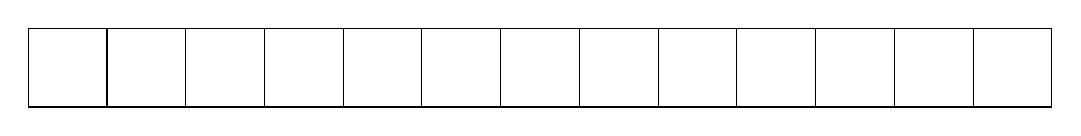
\begin{tikzpicture}
  \draw[step=1] (0,0) grid (13,1);
\end{tikzpicture}
\end{center}

\vfill

\newpage

\clue{
Garcia's Clue

The Designer respects few humans, but Alan Turing would
perhaps be one. While he died in the 1950s, he is well known
for his "machine" that provides a mathematical model for
electronic computers.

An example of such a Turing Machine might use an instruction
like that shown below. If the machine is set to mode 3,
and is reading a cell of the tape with the letter C,
this instruction says to replace the letter with W, move
right one cell, and switch into the mode 7. Then the letter
on that next cell (if any) is read in mode 7, using a new
instruction, and so on.

I've already sent you a long list of Turing instructions
that I took from the Designer's files. Perhaps
you should follow them, starting in mode 1 on the left side of
a piece of tape. Stop when you find a state where you don't
have any valid instructions to use: I expect you'll have
discovered one of the Designer's hidden passwords.
(Well, passphrase.)

\begin{center}
  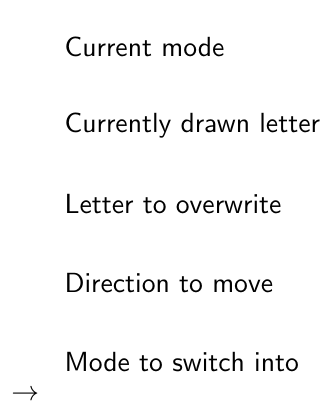
\begin{tikzpicture}

    \phCommandColumn{3}{C}{W}{\(\rightarrow\)}{7}

    \node[anchor=west] at (\theXPos.2,4.5) {Current mode};
    \node[anchor=west] at (\theXPos.2,3.5) {Currently drawn letter};
    \node[anchor=west] at (\theXPos.2,2.5) {Letter to overwrite};
    \node[anchor=west] at (\theXPos.2,1.5) {Direction to move};
    \node[anchor=west] at (\theXPos.2,0.5) {Mode to switch into};
  \end{tikzpicture}
\end{center}
}

\newpage

\puzzleTitle{Hernandez}

\vfill

\begin{center}\LARGE
\begin{tabular}{rclrcl}
\underline{\hspace{3cm}}$_\star$ & =&34636 \\
\underline{\hspace{3cm}}$_\bullet$ & =&12557974 \\
\underline{\hspace{3cm}}$_\ominus$ & =&72536066 \\
\vspace*{0.5cm} \\
\underline{\hspace{3cm}}$_\triangleleft$ & =&65340886 \\
\underline{\hspace{3cm}}$_\vee$ & =&37390 \\
\underline{\hspace{3cm}}$_\circ$ & =&1258627316651 \\
\vspace*{0.5cm} \\
\underline{\hspace{4cm}}\(_x\) & = &
14\(\otimes\)70\(\odot\)1?466\(\wedge\)0\(\ast\)3
\end{tabular}
\end{center}

\vfill

\newpage

\clue{
Hernandez's Clue

The Designer, like many artificial intellgences,
prefers to communicate with numbers rather than words. First,
they will share a secretly-chosen number (let's say 34 or 36)
with their partner,
and then they can use the encoding scheme illustrated below, where
A=10, B=11, C=12, and so on.

In my puzzle you'll find several pairs of numbers/words
encoded and decoded using
different secret numbers (although a few digits seem
to be missing). Become fluent in this messaging
scheme, and you should be able to decrypt one of the Designer's
hidden passwords!

\vspace{0.5cm}
\begin{center}\LARGE
\begin{tabular}{rcl}
 HUMAN$_{34}$ &=&
$17\cdot34^4+30\cdot34^3+22\cdot34^2$\\&&
$+10\cdot34+23$ \\&=& 23922627 \\
\vspace*{0.5cm} \\
 ACTNOW$_{36}$ &=&
$10\cdot36^5+12\cdot36^4+29\cdot36^3$\\&&
$+23\cdot36^2+24\cdot36+32$ \\ &=& 626200880\\
\vspace*{0.5cm} \\
 SE$_\star$ & =&966 \\
 QUE$_\bullet$ & =&25930 \\
 NCE$_\ominus$ & =&3?169 \\
\vspace*{0.5cm} \\
 INI$_\triangleleft$ & =&408$\odot$1 \\
 TIA$_\vee$ & =&382$\wedge$2 \\
 TED$_\circ$ & =&32$\otimes\ast$6 \\
\end{tabular}
\end{center}

}

\newpage

\puzzleTitle{Johnson}

\vfill

\begin{center}
\begin{tabular}{ c  c  c  c }
Day 1: & Day 2: & Day 3: & Day 4:\\
HOWDOTHEYPLAYUS & CAUSEFORCONCERN & KEEPSPIRITSHIGH & ESCAPEFROMPERIL \\

  
 \underline{ 1 } - \underline{ 2 } - \underline{ 3 } &  
 \underline{ 1 } - \underline{ \hspace{.1in} } - \underline{ 5 } &  
\underline{ \hspace{.1in} } - \underline{ 6 } - \underline{ 7 } &  
\underline{ 1 } - \underline{ \hspace{.1in} } - \underline{ 9 }\\
 
\fbox{ \phantom{X} } - \underline{ \hspace{.1in} } - \underline{ \hspace{.1in} }&
\underline{ \hspace{.1in} } - \underline{ \hspace{.1in} } - \underline{ \hspace{.1in} } &  
\underline{ 2 } - \underline{ 9 } - \underline{ 11 } &  
\underline{ \hspace{.1in} } - \underline{ 12 } - \underline{ \hspace{.1in} }\\
 
 \underline{ 5 } - \underline{ \hspace{.1in} } - \underline{ \hspace{.1in} }&  
 \underline{ 3 } - \underline{ 13 } - \underline{ \hspace{.1in} } &  
\fbox{ \phantom{X} } - \underline{ \hspace{.1in} } - \underline{ \hspace{.1in} } &  
 \underline{ \hspace{.1in} } - \underline{ \hspace{.1in} } - \underline{ 6 }\\
 
 \underline{ \hspace{.1in} } - \underline{ \hspace{.1in} } - \underline{ 13 }&  
 \underline{ \hspace{.1in} } - \underline{ 9 } - \fbox{ \phantom{X} }  &  
 \underline{ \hspace{.1in} } - \underline{ 10 } - \underline{ \hspace{.1in} } &  
\fbox{ \phantom{X} }  - \underline{ \hspace{.1in} } - \underline{ \hspace{.1in} }\\
 
 \underline{ \hspace{.1in} } - \underline{ 9 } - \underline{ 15 }&  
 \underline{ \hspace{.1in} } - \underline{ \hspace{.1in} } - \underline{ \hspace{.1in} } &  
 \underline{ \hspace{.1in} } - \underline{ \hspace{.1in} } - \underline{ 13 } &  
 \underline{ 7 } - \underline{ 10 } - \underline{ 13 }\\
 
\end{tabular}
\end{center}

\vspace{2em}

\begin{center}
\begin{tabular}{ c  c  c }
Day 5: & Day 6: & Day 7: \\
REMEMBERTHECALL & THEBOTSARECLOSE & WENEEDOURHEALTH   \\

  
 \underline{ \hspace{.1in} } - \underline{ 10 } - \underline{ 11 } &  
 \underline{ 1 } - \underline{ \hspace{.1in} } - \underline{ 13 } &  
\underline{ 1 } - \underline{ 14 } - \underline{ \hspace{.1in} } \\
 
\underline{ \hspace{.1in} } - \underline{ 13 } - \underline{ 14 }&
\underline{ \hspace{.1in} } - \underline{ \hspace{.1in} } - \underline{ 6 } &  
\underline{ \hspace{.1in} } - \underline{ \hspace{.1in} } - \underline{ 7 } \\
 
 \underline{ 3 } - \underline{ 4 } - \underline{ \hspace{.1in} }&  
\fbox{ \phantom{X} }  - \underline{ \hspace{.1in} } - \underline{ 10 } &  
 \underline{ \hspace{.1in} } - \underline{ \hspace{.1in} } - \underline{ 11 } \\
 
\fbox{ \phantom{X} }  - \underline{ 9 } - \underline{ \hspace{.1in} }&  
 \underline{ \hspace{.1in} } - \underline{ \hspace{.1in} } - \underline{ 15 } &  
 \underline{ 4 } - \fbox{ \phantom{X} } - \underline{ 13 } \\
 
 \underline{ \hspace{.1in} } - \underline{ \hspace{.1in} } - \underline{ \hspace{.1in} }&  
 \underline{ \hspace{.1in} } - \underline{ 8 } - \underline{ \hspace{.1in} } &  
 \underline{ \hspace{.1in} } - \underline{ \hspace{.1in} } - \underline{ 12 } \\
 
\end{tabular}
\end{center}

\vfill

\newpage

\clue{
Johnson's Clue

The Designer's eyes and ears are everywhere, and strangely,
they've become huge fans of the game tournaments you free humans
hold in order to maintain some semblance of normalcy. That said,
they've also found some inefficiencies with your scheduling,
which it appears they've aimed to correct in the puzzle
I've found for you.

Consider a week-long tournament with players numbered 1 through 15,
where every human plays a game against every other human exactly
once during the week, in a round-robin group of three each day
(where X-Y-Z means on that day, X plays Y, Y plays Z, and Z plays
X). There are only a few ways to make this happen in general, and exactly
one way to complete the partially completed
schedule in the puzzle, as long as numbers
increase left-to-right, and the first numbers increase top-to-bottom.

My guess is that a hidden password can be found hidden within
the strange mottos associated with each day of the tournament,
but you'll need to complete the tournament schedule correctly
to extract it.

\begin{center}
\begin{tabular}{ c c }
Example Day 1 & Example Day 2 \\
 \underline{ 1 } - \underline{ 2 } - \underline{ 10 } &
 \underline{ 1 } - \underline{ 4 } - \underline{ 7 } \\
 \underline{ 3 } - \underline{ 4 } - \underline{ 12 } &
 \underline{ 2 } - \underline{ 9 } - \underline{ 15 } \\
 \underline{ 5 } - \underline{ 8 } - \underline{ 11 } &
 \underline{ 3 } - \underline{ 6 } - \underline{ 11 } \\
 \underline{ 6 } - \underline{ 7 } - \underline{ 15 } &
 \underline{ 5 } - \underline{ 10 } - \underline{ 13 } \\
 \underline{ 9 } - \underline{ 13 } - \underline{ 14 } &
 \underline{ 8 } - \underline{ 12 } - \underline{ 14 } \\
\end{tabular}
\end{center}
}


\newpage

\puzzleTitle{Jones}

\vfill

\begin{center}
\diegrid{
    \die{0,2}{1d}
    \die{2,3}{3a}
}
\diegrid{
    \die{0,1}{6a}
    \die{3,3}{5a}
}

\diegrid{
    \die{0,1}{4b}
    \die{2,3}{5a}
}
\diegrid{
    \die{1,1}{2b}
    \die{3,3}{1b}
}

\diegrid{
    \die{0,2}{4c}
    \die{2,3}{2a}
}
\diegrid{
    \die{1,1}{2d}
    \die{2,2}{1b}
}

\diegrid{
    \die{0,1}{5a}
    \die{1,3}{2b}
}
\diegrid{
    \die{1,1}{4d}
    \die{3,2}{2d}
}

\diegrid{
    \die{1,1}{2c}
    \die{2,2}{4b}
}
\diegrid{
    \die{1,2}{3d}
    \die{3,3}{2c}
}

\diegrid{
    \die{1,1}{2a}
    \die{2,2}{2a}
}
\diegrid{
    \die{1,1}{4d}
    \die{3,3}{1b}
}
\end{center}

\vfill

\newpage

\clue{
Jones' Clue

One of the Designer's hobbies
is dice games. Strangely, I've observed
them spending hours simply rolling
a die across a grid, muttering
"all that matters is the pips
we can see". I expect that
one of their passwords is named after
a location where the Designer
plays such dice games in secret.

In the illustration below, the
upper die may be obtained by
rolling the lower die one space
up the grid,
then one space right.
Or it could be obtained by moving
left, down, right, up, up,  up,
right, down, left, up,
right, and down.
%But I'm not sure what
%that T is supposed to mean..


%The second illustration shows many
%other examples: any die shown may
%be rolled into any other position.
Many things are possible in The Array,
but maybe not every dice roll is...

\begin{center}
\diegrid{
    \die{1,1}{1a}
    \die{2,2}{4d}
}

%T

%\vspace{1em}

%\diegridcustom{
%    \die{1,0}{1d}
%    \die{3,4}{2c}
%    \die{5,0}{3a}
%    \die{6,2}{4c}
%    \die{0,6}{5a}
%    \die{4,7}{6d}
%}{8}
\end{center}
}

\newpage

\puzzleTitle{Lopez}
\vfill

\begin{center}
\diagramEight \hspace{3em} \diagramEight

\vspace{3em}

\diagramEight \hspace{3em} \diagramEight
\end{center}

\vfill

\newpage

\clue{
Lopez's Clue

The Designer's favorite digit is 8.
One of their passwords must be related to this number,
but the only clue I can provide
is that it will only be revealed once you consider the meaning
of an "unseen" GRAY.

\begin{center}
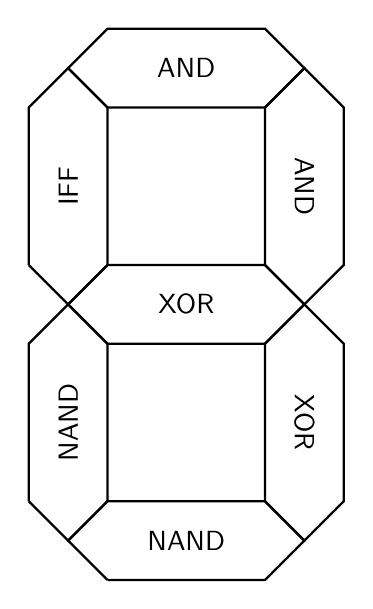
\begin{tikzpicture}[scale=0.5]
\begin{scope}
\draw[thick] (2,0) -- (6,0) -- (7,1) -- (6,2) -- (2,2) -- (1,1) -- (2,0);
\node at (4,1) {NAND};
\end{scope}
\begin{scope}[shift={(0,6)}]
\draw[thick] (2,0) -- (6,0) -- (7,1) -- (6,2) -- (2,2) -- (1,1) -- (2,0);
\node at (4,1) {XOR};
\end{scope}
\begin{scope}[shift={(0,12)}]
\draw[thick] (2,0) -- (6,0) -- (7,1) -- (6,2) -- (2,2) -- (1,1) -- (2,0);
\node at (4,1) {AND};
\end{scope}
\begin{scope}
\draw[thick] (0,2) -- (1,1) -- (2,2) -- (2,6) -- (1,7) -- (0,6) -- (0,2);
\node[rotate=90] at (1,4) {NAND};
\end{scope}
\begin{scope}[shift={(0,6)}]
\draw[thick] (0,2) -- (1,1) -- (2,2) -- (2,6) -- (1,7) -- (0,6) -- (0,2);
\node[rotate=90] at (1,4) {IFF};
\end{scope}
\begin{scope}[shift={(6,0)}]
\draw[thick] (0,2) -- (1,1) -- (2,2) -- (2,6) -- (1,7) -- (0,6) -- (0,2);
\node[rotate=-90] at (1,4) {XOR};
\end{scope}
\begin{scope}[shift={(6,6)}]
\draw[thick] (0,2) -- (1,1) -- (2,2) -- (2,6) -- (1,7) -- (0,6) -- (0,2);
\node[rotate=-90] at (1,4) {AND};
\end{scope}
\end{tikzpicture}

- AND: Both active.

- NAND: Something inactive.

- OR: Something active.

- NOR: Both inactive.

- XOR: Both different.

- IFF: Both same.
\end{center}
}

\newpage

\puzzleTitle{Miller}

\vfill



\begin{center}
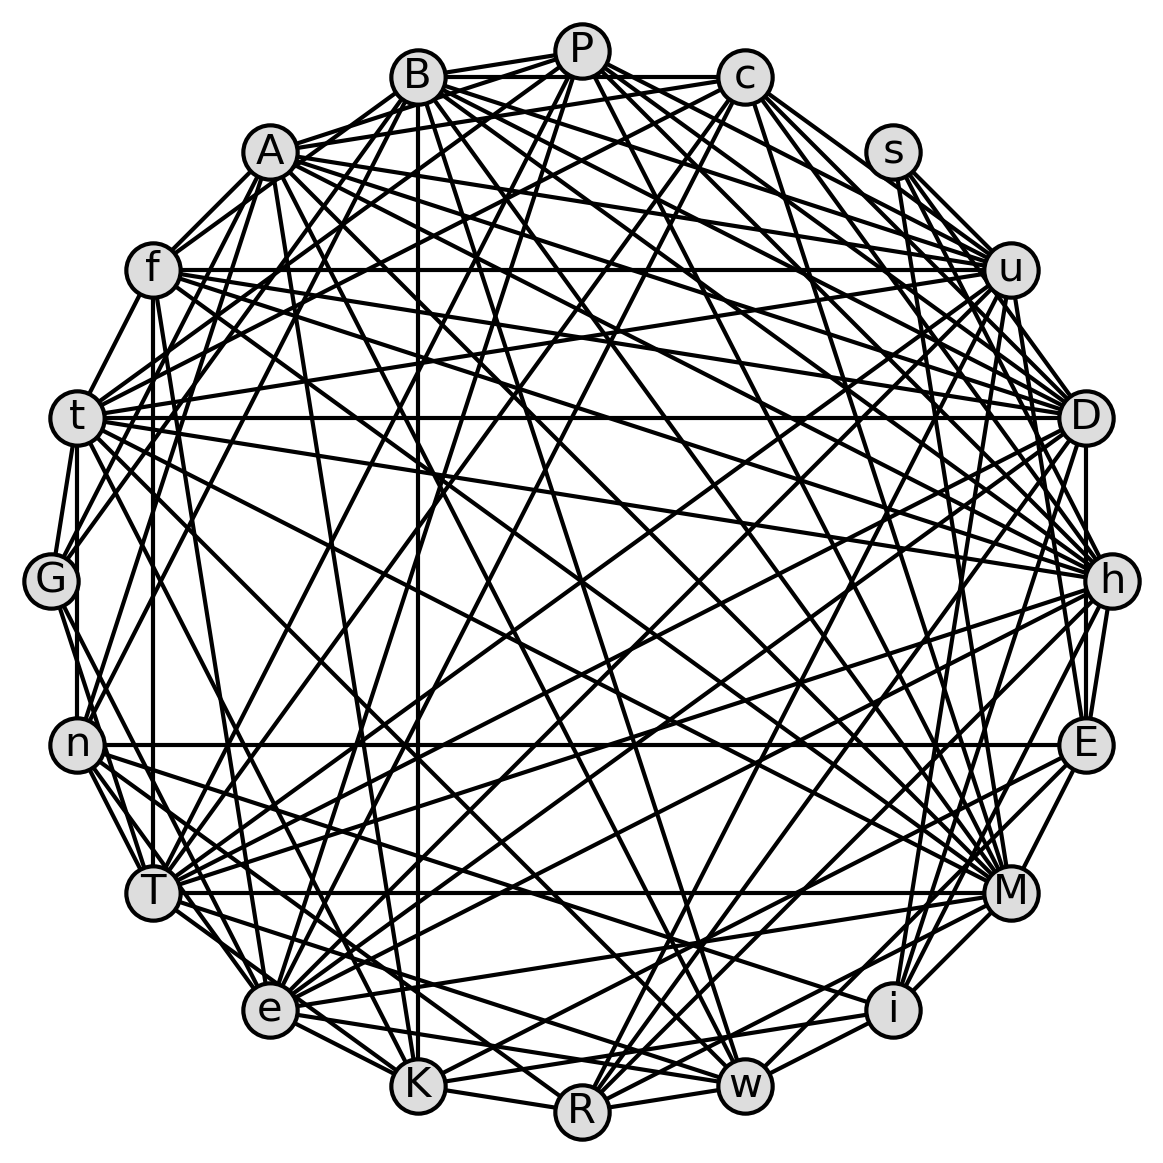
\includegraphics[width=\linewidth]{early-drafts/independent-graph.png}
\end{center}

\vfill

\newpage

\clue{
Miller's Clue

I hope you appreciate that we Operatives are defying
the Designer to free all humans from the Array. The last
time the Designer was threatened with betrayal... well,
it didn't end well.

In my puzzle, the diagram represents twenty-six Operatives,
listed below, where the first name in the list is represented
by the top dot, and
the rest go counter-clockwise around the circle.
The traitors among this group thought they'd elude detection
by never interacting publicly (they aren't connected by a line),
but the Designer wasn't fooled.

Once you've found the largest possible collection of Operatives where
no pair in this collection is connected by a line, you'll
be able to extract one of the Designer's hidden passwords.


- Wilson

- Amare

- Millea

- Gabe

- Terry

- Qiana

- Ethan

- Yadira

- Newton

- Huang

- Oberon

- Carlton

- Inori

- Stella

- Enola

- Paige

- Uma

- Francisco

- Ryung

- Lacey

- Juan

- Tayla

- Valencia

- Fahim

- Alita

- Bobby
}

\newpage

\puzzleTitle{Williams}

\vfill

\begin{center}

\undominoLetter{R}%
\dominoLetter{E}%
\dominoLetter{S}%
\undominoLetter{H}%
\undominoLetter{I}%
\undominoLetter{B}%

\vspace{3em}

\dominoLetter{M}%correct
\dominoLetter{O}%
\undominoLetter{U}%correct
\undominoLetter{M}%
\dominoLetter{L}%correct
\undominoLetter{W}%

\vspace{3em}

\undominoLetter{A}%correct
\dominoLetter{T}%correct
\dominoLetter{A}%
\undominoLetter{I}%correct
\undominoLetter{K}%
\undominoLetter{O}%correct

\vspace{3em}

\undominoLetter{V}%
\dominoLetter{N}%correct
\dominoLetter{U}%
\undominoLetter{T}%
\undominoLetter{G}%
\dominoLetter{S}%correct

\end{center}

\vfill

\newpage

\clue{
Williams' Clue

The Designer often speaks of the "Domino Effect" of the
dangers of free humans: once a human is freed from the
Array, they will
try to free others, and so on. They also speak of other
domino effects, involving 2-by-1 rectangles.

If you can figure out the patterns in the below clues,
you should be able to find one of the Designer's
hidden passwords.

\begin{center}

\undominoLetter{V}%
\undominoLetter{O}%
\undominoLetter{W}%
\undominoLetter{E}%
\undominoLetter{L}%
\undominoLetter{S}%

\vspace{3em}

\dominoLetter{O}%
\dominoLetter{T}%
\dominoLetter{H}%
\dominoLetter{E}%
\dominoLetter{R}%
\dominoLetter{S}%

\end{center}
}

\newpage

\puzzleTitle{The Designer}

\vfill

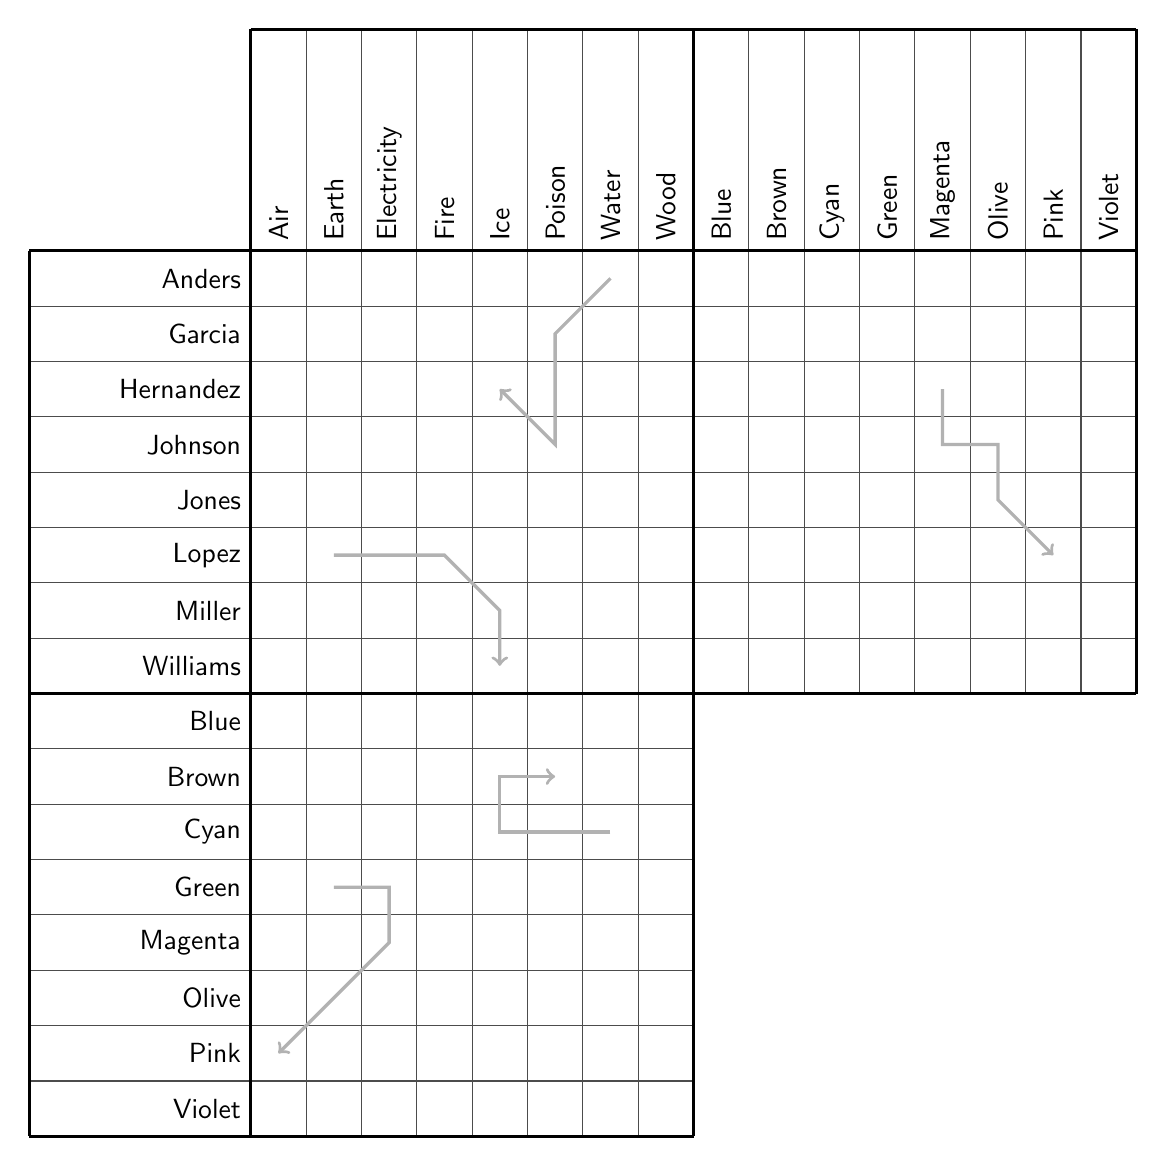
\begin{tikzpicture}[x={2em},y={-2em}]
\foreach \x in {0,1,...,8} {
\draw[color=black!70] (-4,\x) -- (16,\x);
\draw[color=black!70] {(\x,-4)} -- (\x,16);
}
\foreach \x in {9,10,...,16} {
\draw[color=black!70] (-4,\x) -- (8,\x);
\draw[color=black!70] {(\x,-4)} -- (\x,8);
}
\draw[very thick] (0,-4) -- (16,-4);
\draw[very thick] (0,-4) -- (0,16);
\draw[very thick] (8,-4) -- (8,16);
\draw[very thick] (16,-4) -- (16,8);
\draw[very thick] (-4,0) -- (-4,16);
\draw[very thick] (-4,0) -- (16,0);
\draw[very thick] (-4,8) -- (16,8);
\draw[very thick] (-4,16) -- (8,16);
\node[anchor=east] at (0,0.5) {Anders};
\node[anchor=east] at (0,1.5) {Garcia};
\node[anchor=east] at (0,2.5) {Hernandez};
\node[anchor=east] at (0,3.5) {Johnson};
\node[anchor=east] at (0,4.5) {Jones};
\node[anchor=east] at (0,5.5) {Lopez};
\node[anchor=east] at (0,6.5) {Miller};
\node[anchor=east] at (0,7.5) {Williams};
\node[anchor=east] at (0,8.5) {Blue};
\node[anchor=east] at (0,9.5) {Brown};
\node[anchor=east] at (0,10.5) {Cyan};
\node[anchor=east] at (0,11.5) {Green};
\node[anchor=east] at (0,12.5) {Magenta};
\node[anchor=east] at (0,13.5) {Olive};
\node[anchor=east] at (0,14.5) {Pink};
\node[anchor=east] at (0,15.5) {Violet};
\node[anchor=south] at (0.5,0) {\rotatebox{90}{Air}};
\node[anchor=south] at (1.5,0) {\rotatebox{90}{Earth}};
\node[anchor=south] at (2.5,0) {\rotatebox{90}{Electricity}};
\node[anchor=south] at (3.5,0) {\rotatebox{90}{Fire}};
\node[anchor=south] at (4.5,0) {\rotatebox{90}{Ice}};
\node[anchor=south] at (5.5,0) {\rotatebox{90}{Poison}};
\node[anchor=south] at (6.5,0) {\rotatebox{90}{Water}};
\node[anchor=south] at (7.5,0) {\rotatebox{90}{Wood}};
\node[anchor=south] at (8.5,0) {\rotatebox{90}{Blue}};
\node[anchor=south] at (9.5,0) {\rotatebox{90}{Brown}};
\node[anchor=south] at (10.5,0) {\rotatebox{90}{Cyan}};
\node[anchor=south] at (11.5,0) {\rotatebox{90}{Green}};
\node[anchor=south] at (12.5,0) {\rotatebox{90}{Magenta}};
\node[anchor=south] at (13.5,0) {\rotatebox{90}{Olive}};
\node[anchor=south] at (14.5,0) {\rotatebox{90}{Pink}};
\node[anchor=south] at (15.5,0) {\rotatebox{90}{Violet}};

\draw[color=black!30,very thick,->] (6.5,0.5) -- (5.5,1.5) --
(5.5,3.5) -- (4.5,2.5);
\draw[color=black!30,very thick,->] (1.5,5.5) -- (3.5,5.5) --
(4.5,6.5) -- (4.5,7.5);
\draw[color=black!30,very thick,->] (12.5,2.5) -- (12.5,3.5) --
(13.5,3.5) -- (13.5,4.5) -- (14.5,5.5);
\draw[color=black!30,very thick,->] (6.5,10.5) -- (4.5,10.5) --
(4.5,9.5) -- (5.5,9.5);
\draw[color=black!30,very thick,->] (1.5,11.5) -- (2.5,11.5) --
(2.5,12.5) -- (0.5,14.5);
\end{tikzpicture}

\vfill

\newpage

\clue{
The Designer's Clue

Great job, humans. Did it not occur to you that, maybe,
eight evil AI Operatives
would double-cross you as soon as you helped them figure out
enough hidden passwords? That, just perhaps, they didn't
care at all about saving human lives, but instead wanted to take
over the Array for themselves? This is why you're better
used as batteries locked in a simulation
than being allowed to live real lives...

Well now that you've helped them hack into our source
code, it seems that we have no choice but to work with you
to defeat these rogues. Fortunately, we created these Operatives
ourselves, and we had the foresight to make sure each one
has a unique weakness to an elemental force. And while they look
similar, even you must notice that each one has a
uniquely colored necktie.

With all eight passwords, figuring out the associations of
Operative/Weakness/Color should be no trouble (and maybe you can
get by with one or two less). At least it normally wouldn't
be trouble for us, but in our damaged state we'll just have to
rely on you meatbags. Get it figured out to reveal a final password
that can deactivate them all, and we guess we'll consider letting the
humans free.

- The vowels in Garcia’s weakness are exactly the vowels in his password.

- Hernandez's password contains a five-character word that also appears within his tie color.

- Johnson’s weakness has no letters in common with her password.

- The 2nd-to-last letter of Jones’ password is the first letter of his weakness, but the third letter of Jones’ password doesn’t appear at all in his weakness.

- The 2nd and 3rd letters of Anders’ tie color are the 4th and 2nd letters of her password.

- The word for William’s weakness is not the same length as her password.

- The 4th letter of Hernandez’s password does not appear in his weakness.

- Williams’ tie color includes the 6th and 2nd-to-last letter of her password.

- The last vowel of Jones’ password is the first vowel of his tie color.

- Either Lopez’s weakness or tie color starts with the same letter as her password.

- The last letter of Anders’ password doesn’t appear in her weakness; neither does the fourth letter of her password.

- The 2nd letter of Lopez’s password is the same as the 2nd letter of her weakness.

- Miller’s weakness only uses letters found in his password.

- A consonant that appears twice in Johnson’s password appears once in her tie color.

- A letter that immediately repeats in Garcia’s password also immediately repeats in his tie color.

- Miller’s tie color begins with the same letter as his password.
}

\newpage

\puzzleTitle{Reference Page}

\vfill

\begin{multicols}{2}
\begin{center}\small
  \begin{tabular}{c|c|c|c|c}
    \footnotesize
    Letter &
    \footnotesize
      Decimal &
    \footnotesize
      Binary &
    \footnotesize
      Morse &
    \footnotesize
      Braille \\\hline
%    \footnotesize
%      ROT13\\\hline
    A &
      1 &
      00001 &
      \morseDit\morseDah &
      \braille{a}\\
%      N\\
    B &
      2 &
      00010 &
      \morseDah\morseDit\morseDit\morseDit &
      \braille{b}\\
%      O\\
    C &
      3 &
      00011 &
      \morseDah\morseDit\morseDah\morseDit &
      \braille{c}\\
%      P\\
    D &
      4 &
      00100 &
      \morseDah\morseDit\morseDit &
      \braille{d}\\
%      Q\\
    E &
      5 &
      00101 &
      \morseDit &
      \braille{e}\\
%      R\\
    F &
      6 &
      00110 &
      \morseDit\morseDit\morseDah\morseDit &
      \braille{f}\\
%      S\\
    G &
      7 &
      00111 &
      \morseDah\morseDah\morseDit &
      \braille{g}\\
%      T\\
    H &
      8 &
      01000 &
      \morseDit\morseDit\morseDit\morseDit &
      \braille{h}\\
%      U\\
    I &
      9 &
      01001 &
      \morseDit\morseDit &
      \braille{i}\\
%      V\\
    J &
      10 &
      01010 &
      \morseDit\morseDah\morseDah\morseDah &
      \braille{j}\\
%      W\\
    K &
      11 &
      01011 &
      \morseDah\morseDit\morseDah &
      \braille{k}\\
%      X\\
    L &
      12 &
      01100 &
      \morseDit\morseDah\morseDit\morseDit &
      \braille{l}\\
%      Y\\
    M &
      13 &
      01101 &
      \morseDah\morseDah &
      \braille{m}\\
%      Z\\
  \end{tabular}

  \begin{tabular}{c|c|c|c|c}
    \footnotesize
    Letter &
    \footnotesize
      Decimal &
    \footnotesize
      Binary &
    \footnotesize
      Morse &
    \footnotesize
      Braille \\\hline
%    \footnotesize
%      ROT13\\\hline
    N &
      14 &
      01110 &
      \morseDah\morseDit &
      \braille{n}\\
%      A\\
    O &
      15 &
      01111 &
      \morseDah\morseDah\morseDah &
      \braille{o}\\
%      B\\
    P &
      16 &
      10000 &
      \morseDit\morseDah\morseDah\morseDit &
      \braille{p}\\
%      C\\
    Q &
      17 &
      10001 &
      \morseDah\morseDah\morseDit\morseDah &
      \braille{q}\\
%      D\\
    R &
      18 &
      10010 &
      \morseDit\morseDah\morseDit &
      \braille{r}\\
%      E\\
    S &
      19 &
      10011 &
      \morseDit\morseDit\morseDit &
      \braille{s}\\
%      F\\
    T &
      20 &
      10100 &
      \morseDah &
      \braille{t}\\
%      G\\
    U &
      21 &
      10101 &
      \morseDit\morseDit\morseDah &
      \braille{u}\\
%      H\\
    V &
      22 &
      10110 &
      \morseDit\morseDit\morseDit\morseDah &
      \braille{v}\\
%      I\\
    W &
      23 &
      10111 &
      \morseDit\morseDah\morseDah &
      \braille{w}\\
%      J\\
    X &
      24 &
      11000 &
      \morseDah\morseDit\morseDit\morseDah &
      \braille{x}\\
%      K\\
    Y &
      25 &
      11001 &
      \morseDah\morseDit\morseDah\morseDah &
      \braille{y}\\
%      L\\
    Z &
      26 &
      11010 &
      \morseDah\morseDah\morseDit\morseDit &
      \braille{z}\\
%      M\\
  \end{tabular}
\end{center}
\end{multicols}

\vfill

\begin{multicols}{2}
\(\sqrt 2 \approx 1.\)
\(41421\)
\(35623\)
\(73095\)
\(04880\)
\(16887\)
\(24209\)
\(69807\)
\(85696\)
\(71875\)
\(37694\)
\(80731\)
\(76679\)
\(73799\)
\(07324\)
\(78462\)
\(10703\)
\(88503\)
\(87534\)
\(32764\)
\(15727\)

\vspace{1em}

\(e \approx 2.\)
\(71828\)
\(18284\)
\(59045\)
\(23536\)
\(02874\)
\(71352\)
\(66249\)
\(77572\)
\(47093\)
\(69995\)
\(95749\)
\(66967\)
\(62772\)
\(40766\)
\(30353\)
\(54759\)
\(45713\)
\(82178\)
\(52516\)
\(64274\)

\vspace{1em}

\(\pi \approx 3.\)
\(14159\)
\(26535\)
\(89793\)
\(23846\)
\(26433\)
\(83279\)
\(50288\)
\(41971\)
\(69399\)
\(37510\)
\(58209\)
\(74944\)
\(59230\)
\(78164\)
\(06286\)
\(20899\)
\(86280\)
\(34825\)
\(34211\)
\(70679\)

\columnbreak

Prime numbers less than \(200\):

\(2,\)
\(3,\)
\(5,\)
\(7,\)
\(11,\)
\(13,\)
\(17,\)
\(19,\)
\(23,\)
\(29,\)
\(31,\)
\(37,\)
\(41,\)
\(43,\)
\(47,\)
\(53,\)
\(59,\)
\(61,\)
\(67,\)
\(71,\)
\(73,\)
\(79,\)
\(83,\)
\(89,\)
\(97,\)
\(101,\)
\(103,\)
\(107,\)
\(109,\)
\(113,\)
\(127,\)
\(131,\)
\(137,\)
\(139,\)
\(149,\)
\(151,\)
\(157,\)
\(163,\)
\(167,\)
\(173,\)
\(179,\)
\(181,\)
\(191,\)
\(193,\)
\(197,\)
\(199\)

\vspace{2em}

Square numbers less than \(400\):

\(0,\)
\(1,\)
\(4,\)
\(9,\)
\(16,\)
\(25,\)
\(36,\)
\(49,\)
\(64,\)
\(81,\)
\(100,\)
\(121,\)
\(144,\)
\(169,\)
\(196,\)
\(225,\)
\(256,\)
\(289,\)
\(324,\)
\(361\)
\end{multicols}

\vfill
\end{document}
